\documentclass[12pt,a4paper]{report}
\usepackage[utf8]{inputenc}
\usepackage{amsmath}
\usepackage{amsfonts}
\usepackage{amssymb}
\usepackage{amsthm}
\usepackage{hyperref}

\usepackage{multicol}
\usepackage{fancyhdr}
\usepackage[inline]{enumitem}
\usepackage{tikz}
\usepackage{tikz-cd}
\usetikzlibrary{calc}
\usetikzlibrary{shapes.geometric}
\usetikzlibrary{positioning}
\usepackage[margin=0.5in]{geometry}
\usepackage{xcolor}

\hypersetup{
    colorlinks=true,
    linkcolor=blue,
    filecolor=magenta,      
    urlcolor=cyan,
    pdftitle={Tensors},
    pdfpagemode=FullScreen,
    }

%\urlstyle{same}

\newcommand{\CLASSNAME}{Math 5050 -- Special Topics: Differential Geometry}
\newcommand{\STUDENTNAME}{Paul Carmody}
\newcommand{\ASSIGNMENT}{Section 22: Bounded Manifolds }
\newcommand{\DUEDATE}{October 22, 2025}
\newcommand{\PROFESSOR}{Professor Berchenko-Kogan}
\newcommand{\SEMESTER}{Fall 2025}
\newcommand{\SCHEDULE}{TBD}
\newcommand{\ROOM}{Remote}

\newcommand{\MMN}{M_{m\times n}}
\newcommand{\FF}{\mathcal{F}}

\pagestyle{fancy}
\fancyhf{}
\chead{ \fancyplain{}{\CLASSNAME} }
%\chead{ \fancyplain{}{\STUDENTNAME} }
\rhead{\thepage}
\input{../MyMacros}

\newcommand{\RED}[1]{\textcolor{red}{#1}}
\newcommand{\BLUE}[1]{\textcolor{blue}{#1}}

\newcommand{\SUPP}{\operatorname{supp}}
\newcommand{\CLOSURE}{\operatorname{closure of}}
\newcommand{\BD}{\operatorname{bd}}
\newcommand{\HHN}{\mathcal{H}^n}

\begin{document}

\begin{center}
	\Large{\CLASSNAME -- \SEMESTER} \\
	\large{ w/\PROFESSOR}
\end{center}
\begin{center}
	\STUDENTNAME \\
	\ASSIGNMENT -- \DUEDATE\\
\end{center} 

\textbf{Key Points}

\HLINE
\begin{remark}

Charts map boundary points to boundary points.  That is, $(U, \phi)$ is a chart on $M$ then $p \in \partial M$ implies $\phi(p) \in \partial\phi(U)$.
\end{remark}

\begin{remark}

Topological boundaries/properties are taken from the \textit{ambient} space (as if we are ignoring the manifold that it contains).  Manifold properties are always measured from ``within", that is, proved via the charts within the atlas that fully defines the Manifold.

\end{remark}

\HLINE
\begin{enumerate}[label=22.\arabic*]

\item \textbf{Topological boundary versus manifold boundary}

Let $M$ be the subset $[0,1) \cup \{2\}$ of the real line.  Find its topological boundary $\BD(M)$ and its manifold boundary $\partial M$.

\BLUE{
Since $[0,1)$ is a one dimensional manifold its the boundary must be $\BD([0,1)) = \{0\}$.  The singleton set $\{2\}$ is a zero-dimensional manifold thus has no boundary.
}

\item \textbf{Topological boundary of an intersection}

Let $A$ and $B$ be two subsets of a topological space $S$.  Prove that
\begin{align*}
	\BD(A \cap B) \subset \BD(A) \cup \BD(B).
\end{align*}

\BLUE{Consider a proof by contrapositive, that is, $x\not \in 	\BD(A \cap B) \implies  x\not \in \BD(A) \cup \BD(B)$.  Note that
$\BD(A)^c = A^o\cup S \backslash \CONJ{A}$ then,
\begin{align*}
	x &\in (\BD(A) \cup \BD(B))^c\\
	x &\in \BD(A)^c \cap \BD(B)^c \\
	x &\in A^o\cup S \backslash \CONJ{A} \AND x \in B^o\cup S \backslash \CONJ{B}\\
	x &\not \in \BD(A) \AND x \not \in \BD(B) \\
	\therefore x &\not \in \BD(A \cap B) \subset \BD(A)
\end{align*}
}

\item \textbf{Inward-pointing vectors at the boundary}

Let $M$ be a manifold with boundary and let $p \in \partial M$.  Show that $X_p\in T_pM$ is inward-pointing if and only if in any coordinate chart $(U,x^1,\dots,x^n)$ centered at $p$, the coefficient of $(\PART{}{x^n})_p$ in $X_p$ is positive.

\item \textbf{Smooth outward-pointing vector field along the boundary}

Show that the vector field $X = \sum \rho_\alpha X_\alpha$ defined in the proof of Proposition 22.10 is a smooth outward-pointing vector field along $\partial M$.

\item \textbf{Boundary orientation}

Let $M$ be an oriented manifold with boundary, $\omega$ an orientation form for $M$, and $X$ a $C^\infty$ outward-pointing vector field along $\partial M$.
\begin{enumerate}
	\item if $\tau$ is another orientation form on $M$, then $\tau = f\omega$ for a $C^\infty$ everywhere-positive function $f$ on $M$.  Show that $\iota_X\tau = ft_X\omega$ and therefore, $\iota_X\tau \sim \iota_X\omega$ on $\partial M$.  (Here '$\sim$' is the equivalence relation defined in Subsection 21.4.)
	\item Prove that if $Y$ is another $C^\infty$ outward-pointing vector field along $\partial M$, then $\iota_X\omega \sim \iota_y\omega$ on $\partial M$.
\end{enumerate}

\item \textbf{Induced atlas on the boundary}

Assume $n \ge 2$ and let $(U,\phi)$ and $(V, \psi)$ be two charts in an oriented atlas of an orientable $n$-manifold $M$ with boundary.  Prove that if $U\cap V\cap \partial M\ne 0$, then the restriction of the transition function $\psi\circ\phi^{-1}$ to the boundary $B:= \phi(U\cap V)\cap\partial \HHN$,
\begin{align*}
	(\psi\circ\phi^{-1})|_B: \phi(U\cap V)\cap\partial\HHN\to\psi(U\cap V)\cap\partial\HHN,
\end{align*}has positive Jacobian determinant. (\textit{Hint:} Let $\phi=(x^1,\dots,x^n)$ and $\psi=(y^1,\dots,y^n)$.  Show that the Jacobian matrix of $\phi\circ\phi^{-1}$ in local coordinates is block triangular with $J(\psi\circ\phi^{-1})|_B$ and $\PART{y^n}{x^n}$ as the diagonal blocks, and that $\PART{y^n}{x^n} >0$.)

Thus, if $\{(U_\alpha,\phi_\alpha)\}$ is an oriented atlas for a manifold $m$ with boundary, then the induced atlas $\{(U_\alpha\cap\partial M, \phi_\alpha|_{U_\alpha\cap\partial M})\}$ for $\partial M$ is oriented.


\item \textbf{Boundary orientation of the left half-space}

let $M$ be the left half-space
\begin{align*}
	\{(x^1,\cdots, x^n)\in\R^n\,|\, x^1\le 0\},
\end{align*}with orientation from $dx^1\wedge\cdots\wedge dx^n$.  Show that an orientation from the boundary orientation on $\partial M = \{(0,x^2,\dots,x^n)\in \R^n\}$ is $dx^2\wedge\cdots\wedge dx^n$.

Unlike the upper half-space $\HHN$, whose boundary orientation takes on a sign (Example 22.13), this exercise shows that the bouddary orientation for the left half-space has no sign.  For this reason some authors use the left half-space as the model of a manifold with boundary.

\item \textbf{Boundary orientation on a cylinder}

Let $M$ be the cylinder $S^1\times [0,1]$ with the counterclockwise orientation when viewed from the exterior (Figure 22.7(a)).  Describe the boundary orientation on $C_0=S^1\times\{0\}$ and $C_1=s^1\times \{1\}$.

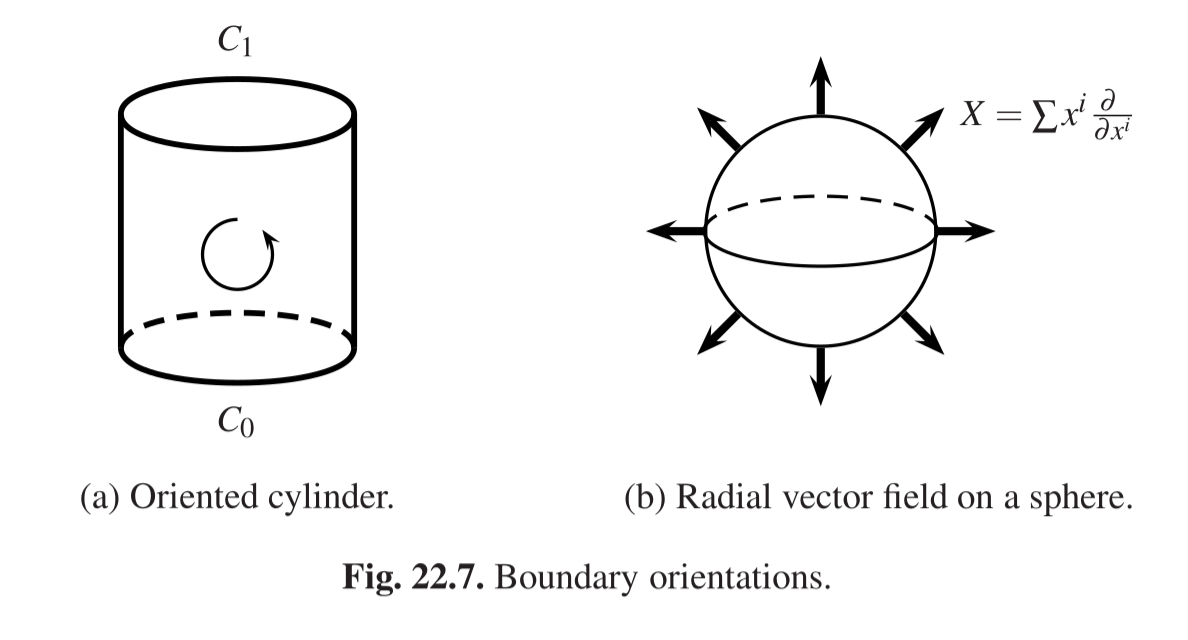
\includegraphics[scale=0.3]{22.7.png} 

\item \textbf{Boundary orientation on a sphere}

Orient the unit sphere $S^n$ in $\R^{n+1}$ as the boundary of the closed unit ball.  Show that an orientation form on $S^n$ is 
\begin{align*}
	\omega &= \sum_{i=1}^{n+1} (-12)^{_i-1} x^i dx^1\wedge\cdots\wedge \hat{d^xi}\wedge\cdots\wedge dx^{x+1},
\end{align*}where the caret $\hat{}$ over $dx^i$ indicates that $dx^i$ is to be omitted. (\textit{Hint: }An outward pointing vector field on $S^n$ is the radial vector field $X=\sum x^i\PART{}{x^i}$ as in Figure 22.7(b).)

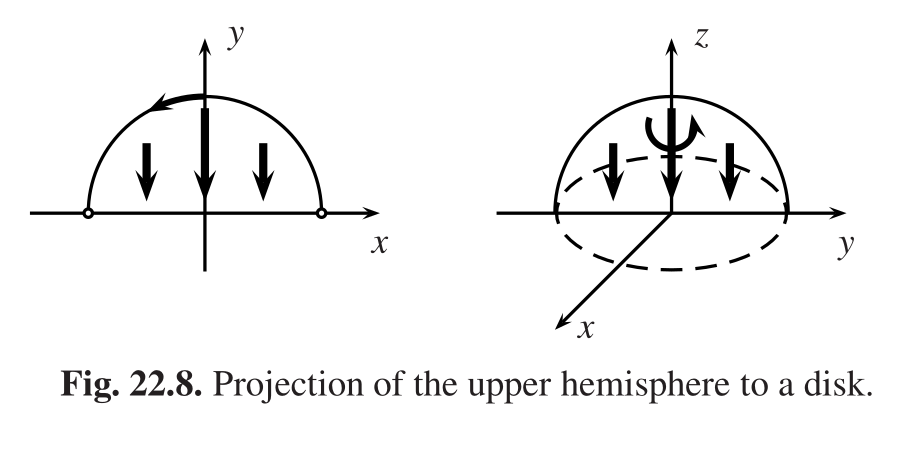
\includegraphics[scale=0.4]{22.8.png} 

\item \textbf{Orientation on the upper hemisphere of a sphere}

Orient the unit sphere $S^n$ in $\R^{n-1}$ as the boundary of the closed unit ball.  Let $U$ be the upper hemisphere
\begin{align*}
	U=\{x\in S^n\,|\,x^{n+1}> 0\}
\end{align*}It has a coordinate chart on the sphere with coordinates $x^1, \dots, x^n$.
\begin{enumerate}
	\item Find an orientation form on $U$ in terms of $dx^1,\dots, dx^n$.
	\item Show that the projection map $\pi: U \to \R^n$.
	\begin{align*}
		\pi(x^1,\dots,x^n,x^{n+1})= (x^1,\dots, x^n),
	\end{align*}is orientation-preserving if and only if $n$ is even (Figure 22.8).
\end{enumerate}

\item \textbf{Antipodal map on a sphere and the orientability of $\R P^n$}

\begin{enumerate}
	\item the antipodal map $a: S^n\to S^n$ on the $n$-sphere is defined by
	\begin{align*}
		a(x^1,\dots,x^n) &= (-x^1,\dots,-x^n)
	\end{align*}Show that the antipodal map is orientation-preserving if and only if $n$ is odd.
	
	\BLUE{The differential is 
	\begin{align*}
		da(x^i) &= -I_{n+1}
	\end{align*}restricting $da$ to the tangent space and taking the determinant
	\begin{align*}
		da_x|_{T_x(S_n)} = -I_{n-1} \\
		\det\PAREN{da_x|_{T_x(S_n)}} &= (-1)^{n-1}
	\end{align*}which is orientation preserving when $n$ is odd and orientation reversing when $n$ is even.
	}
	
	\item Use part (a) and Problem 21.6 to prove that an odd-dimensional real projective space $\R P^n$ is orientable.
\end{enumerate}
\end{enumerate}
\end{document}
